% ------------------------------------------------------------------------
%	Latex Preamble:  Formatting and Custom Commands
% ------------------------------------------------------------------------
\documentclass[12pt]{article}

\usepackage{amsmath, graphicx, subfig}

% to control the page number location and running title
\usepackage{fancyhdr}

% For the draft
\usepackage{endfloat}

% To control the spacing
\usepackage{setspace}

% For including code1
%\usepackage{listings}

% For using s
\usepackage{url}

% Citations are numbers, with round parenthesis
% no brackets around numbers in the bibliography
% use the CBE/CSE bib style
\usepackage[numbers,round]{natbib}
\renewcommand{\bibnumfmt}[1]{#1.}
\bibliographystyle{mrm}

% Equations have square brackets around them
\makeatletter
  \def\tagform@#1{\maketag@@@{[#1]\@@italiccorr}}
\makeatother

% Spacing and indentation
\topmargin -0.4in
\headheight 0.45in
\oddsidemargin 0in
\evensidemargin 0in
\textwidth 6.5in
\textheight 9in

\setlength{\parindent}{0pt} % No paragraph indent.
\setlength{\parsep}{12pt}   % Paragraph separation.
\setlength{\parskip}{12pt}  % Paragraph skip.

% Set the graphics path
\graphicspath{{./figures/}}


% ------------------------------------------------------------------------
%	Document start
% ------------------------------------------------------------------------
\begin{document}

\lhead{ISMRM Raw Data Format}
\chead{}
\rhead{\thepage}
\lfoot{}
\cfoot{}
\rfoot{}

% ------------------------------------------------------------------------
%	Full Title Page
% ------------------------------------------------------------------------
\newpage
\clearpage
\pagestyle{empty}
\vspace*{20mm}

\begin{center}
\large \textbf{ISMRM Raw Data Format: A Proposed Standard for Sharing MRI Raw Datasets}

\normalsize
\singlespacing
Souheil J. Inati$^1$,
Joseph D. Naegele$^1$, 
Nicholas R. Zwart$^2$,
Vinai Roopchansingh$^1$,
Martin J. Lizak$^3$,
David C. Hansen$^4$,
Chia-Ying Liu$^5$,
David Atkinson$^6$,
Peter Kellman$^7$,
Sebastian Kozerke$^8$,
Hui Xue$^7$,
Thomas S. Sorensen$^4$,
James G. Pipe$^2$,
Michael S. Hansen$^7$
\end{center}

\begin{enumerate}
\item National Institute of Mental Health, National Institutes of Health, Bethesda, MD
\item Keller Center for Imaging Innovation, Barrow Neurological Institute, Phoenix, AZ
\item National Institute of Neurologic Disease and Stroke, National Institutes of Health, Bethesda, MD
\item Department of Computer Science, Aarhus University, Aarhus, Denmark
\item Warren Grant Magnusson Clinical Center, National Institutes of Health, Bethesda, MD
\item Centre for Medical Image Computing, University College London, United Kingdom
\item National Heart, Lung, and Blood Institute, National Institutes of Health, Bethesda, MD
\item Institute for Biomedical Engineering, University and ETH Zurich, Zurich, Switzerland
\end{enumerate}

\vspace{5mm}
Correspondence to: \\
Souheil J. Inati \\
National Institue of Mental Health, NIH \\
NIH Building 10/1D-70 \\
10 Center Drive \\
Bethesda, MD 20892 \\
\textit{souheil.inati@nih.gov} \\

\textit{Running Head:  ISMRMRD}

\vspace{5mm}

\textit{Submitted to Magnetic Resonance in Medicine} 

% ------------------------------------------------------------------------
%	Abbreviated Title Page
% ------------------------------------------------------------------------
\newpage
\clearpage
\pagenumbering{arabic} % begin numbering here
\pagestyle{fancy}
\begin{center}
\vspace*{70mm}
\large \textbf{ISMRM Raw Data Format: A Proposed Standard for Sharing MRI Raw Datasets} \\
\end{center}
\normalsize 

\textit{Running Head:  ISMRMRD}

\vspace{5mm}

\textit{Submitted to Magnetic Resonance in Medicine} 

\textit{Word count:  }  

% ------------------------------------------------------------------------
%	Abstract
% ------------------------------------------------------------------------
\newpage
\clearpage
\doublespacing
\section*{Abstract}
\textbf{Purpose:} A common raw data format is a prerequisite for sharing MR image reconstruction algorithms and code, and is a necessary component of reproducible research.  Ideally, this common format would be vendor neutral, and would capture the data fields needed to describe the details of the MR experiment so as to permit image reconstruction from the raw data.  We propose the ISMRM Raw Data (ISMRMRD) format as an example of such a common raw data format, describe its design and implementation, and provide an example of its use in the context of reproducible research.\\
\textbf{Methods:} A file format consisting of a flexible header and tagged frames of k-space data and (optionally) trajectories was designed and  Application Programming Interfaces were implemented in C/C++, MATLAB and Python following an open source development model.  Converters for Bruker, General Electric, Philips and Siemens proprietary file formats were implemented in C++. The library and associated tools were compiled on Linux, Windows and Macintosh computers. Raw data were collected from a phantom on MRI scanners from the four different vendors, converted to ISMRMRD format, and reconstructed using a conventional 2D image reconstruction algorithm implemented in three programming languages (C++, MATLAB, Python).\\
\textbf{Results:} Images obtained by reconstructing the raw data from the four different vendors demonstrate the feasibility of this approach and the utility of the entire toolchain.  The source code, raw data, and images comprising this work were shared online, serving as an example of an image reconstruction project following a paradigm of reproducible research.\\
\textbf{Conclusion:} The proposed raw data format solves a practical problem
for the MRI community.  As this standard is refined, it may serve as a foundation upon which practitioners can base reproducible research and collaborations.  The ISMRMRD format is a completely open and community driven format and we invite members of the community (including commercial vendors) to participate either as users of the format or as developers of the format or associated tools.

\textit{Abstract word count: }  

% ------------------------------------------------------------------------
%	Keywords
% ------------------------------------------------------------------------
\textbf{Keywords:}  Image reconstruction, Open Source, Raw Data Format

% ------------------------------------------------------------------------
%	Body
% ------------------------------------------------------------------------
\newpage
\clearpage
\onecolumn

% ------------------------------------------------------------------------
%	Introduction
% ------------------------------------------------------------------------
\section*{Introduction}
Image reconstruction research has played a pivotal role in driving many advances in magnetic resonance imaging. Examples of paradigm shifting techniques include parallel imaging~\cite{Pruessmann:1999uq, Sodickson:1997fk, Griswold:2002kx}  and more recently the introduction of compressed sensing~\cite{Donoho:2006compressed, Lustig:2007vn}. Novel reconstruction algorithms build on and improve existing methodology and most reconstruction articles compare new methods to existing methods in terms of image quality and reconstruction speed.

Reproducible research has drawn a great deal of attention recently, as highlighted for example in a recent special issue of Science~\cite{Jasny:2011again, Peng:2011reproducible}. The field of computational science in particular has produced several excellent examples of how such research can be carried out, e.g. the wavelab toolbox~\cite{wavelab}.  The ISMRM has begun to take steps to help to facilitate reproducible research, e.g. with the MRI unbound website~\cite{mri_unbound}. Underlying many of these efforts is a discipline specific file format specification that allows scientists to easily exchange data.  Much of modern astronomy research, for example, relies on telescope data in the FITS standard~\cite{fits}.  Other discipline specific data formats have enabled scientists to escape from the limitations imposed by vendor specific proprietary technology, leading to the development of a wide range of post acquisition data analysis tools, and enabling large scale collaborations.  Medical imaging has the DICOM standard~\cite{dicom}, which allows radiology departments to store data from different vendors on a centralized PACS, and computer scientists to implement novel image processing methods in a vendor neutral manner. The subfield of neuroimaging has NIfTI~\cite{nifti}, which underlies large scale projects like the human connectome project~\cite{connectome}.  For the field of MRI, these image file formats serve well, but they do not address the needs of practitioners involved in the development of image reconstruction algorithms, nor do they store the data in a format that is very closely tied to the instrument and to the particulars of the MR experiment. We believe that a first and necessary step is the development of a MR specific raw data file format.

This ISMRMRD standard was developed by a subcommittee of the ISMRM Sedona 2013 workshop.  It is designed to capture the details of the MRI experiment in a way that permits image reconstruction.  It is important to note that this goal is fundamentally different from that of proprietary vendor raw data file formats.  Generally speaking, proprietary vendor raw file formats are intended to capture protocol parameters and the state of the scanner graphical user interface (GUI) for a particular pulse sequence at the time of the scan.  The proprietary vendor raw data file formats are intended to store the information needed to reproduce a particular experiment on a specific version of the scanner software version, and to enable image reconstruction within that same scanner's image reconstruction software framework.  Because of the tight coupling between 1) the scanner console user interface, 2) the pulse sequence and the pulse sequence control parameters, and 3) the image reconstruction software and the image reconstruction software control parameters, the  vendor raw data file formats depend on and contain a great deal of proprietary vendor specific knowledge making them unsuitable for data sharing.  More importantly, the specific implementation details of a particular vendor's scanner software architecture greatly influences the design of these file formats and the type of information that they contain.  The ISMRMRD standard on the other hand is designed to permit the exchange of the raw k-space data and a description of the physics of the data acquisition process, at least in so far as image reconstruction is concerned.

While the ISMRMRD format will continue to evolve as it attracts more users with a more diverse set of applications and needs, the basic format has remained stable enough for a while that it makes sense to present it to the MRI community. This papers lays out the basic design and structure of the format and it also describes several software tools that have been developed to interact with data in ISMRMRD format. A number of vendor specific tools have been created for converting proprietary data formats to this new open standard. We provide an overview of the current status of these data converters and information needed to locate them. As a demonstration of how the data format can be used, a phantom has been scanned on four different scanners and converted to ISMRMRD and been reconstructed with generic, vendor independent reconstruction programs written in Matlab, Python, and C++ programming languages. 

All software, data, figures, scripts to generate the figures, and the text itself contained in this manuscript are available as open source. 


% ------------------------------------------------------------------------
%	Methods
% ------------------------------------------------------------------------
\section*{Architecture and Implementation}
\subsection*{Design}
The ISMRMRD format combines a mix of flexible data structures (XML header) and fixed structures (equivalent to C-structs).  A minimal raw data set is depicted in fig.~\ref{fig:format} and consists of two sections:
\begin{itemize}
\item{XML header.} A flexible XML format document that can contain an arbitrary number of fields and accommodate everything from simple values (matrix sizes, etc.) to entire vendor protocols, etc. This purpose of this XML document is to provide parameters that may be meaningful for some experiments but not for others. This XML format is defined by an XML Schema Definition file (ismrmrd.xsd).
\item{Raw data.} This section contains all the acquired data in the experiment organized as a sequence of data items.  Each data item corresponds to a single frame or chunk in an experiment, for example a single line of data in a cartesian acquisition or a single interleave in a multi-shot spiral acquisition. Each data item consists of a fixed size header (C-struct) with encoding numbers, etc., along with the k-space data for all of the acquired channesl, and (optionally) the k-space trajectory as depicted in fig.~\ref{fig:cstruct}. The raw data structures are defined in a C/C++ header file (ismrmrd.h).
\end{itemize}
The format also provides a simple image format for storing the product of reconstructions and a multi-dimensional array format for storing additional user-specified parameters (e.g. gradient non-linearity correction maps, etc.).

% Figure 1
\begin{figure}
\begin{center}
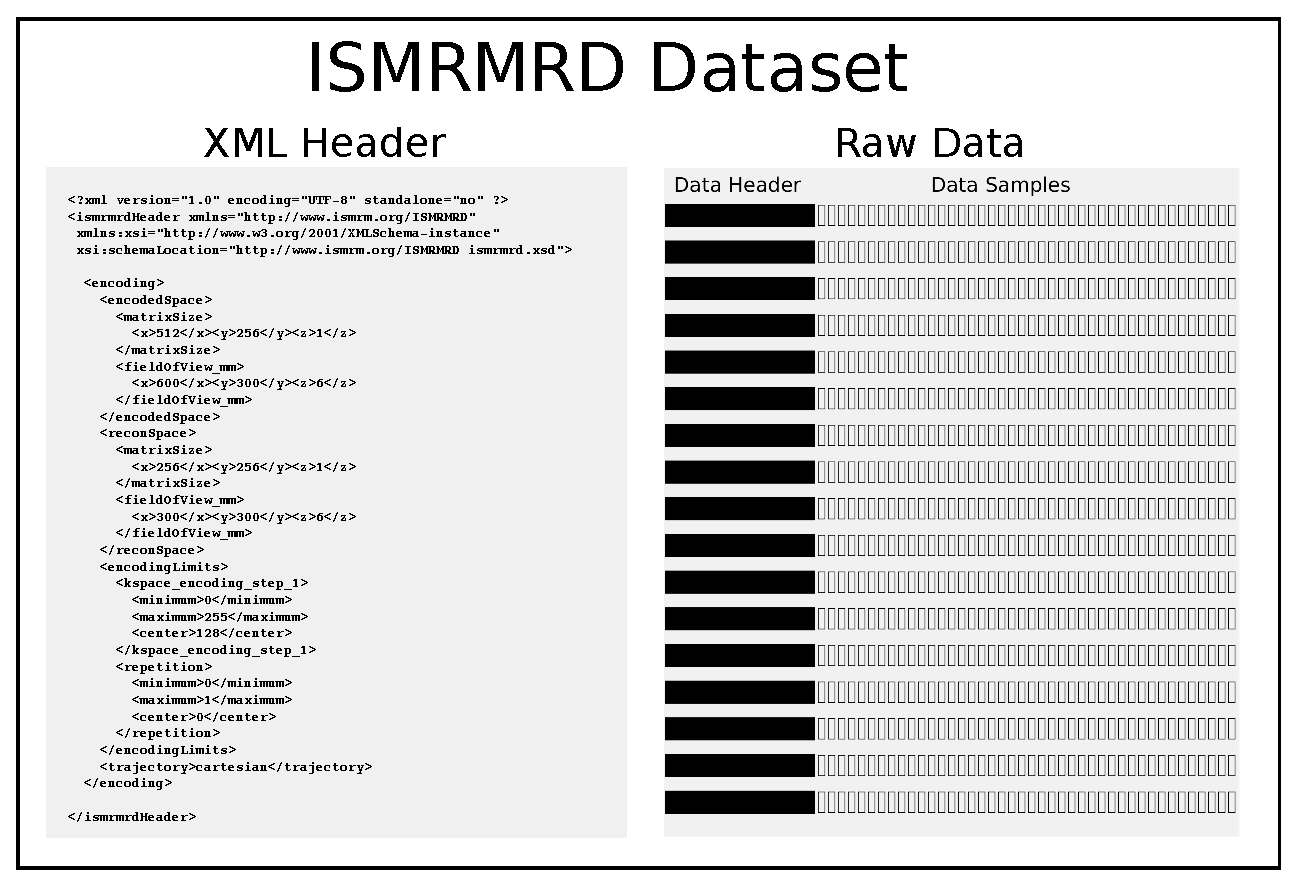
\includegraphics[width=6in]{figure1_ismrmrd_format.eps}
\caption{Minimal ISMRMRD dataset consists of a flexible XML header and raw data organized as sequence of data items consisting of a fixed data header and the k-space data samples}
\label{fig:format}
\end{center}
\end{figure}

% Figure 2
\begin{figure}
\begin{center}
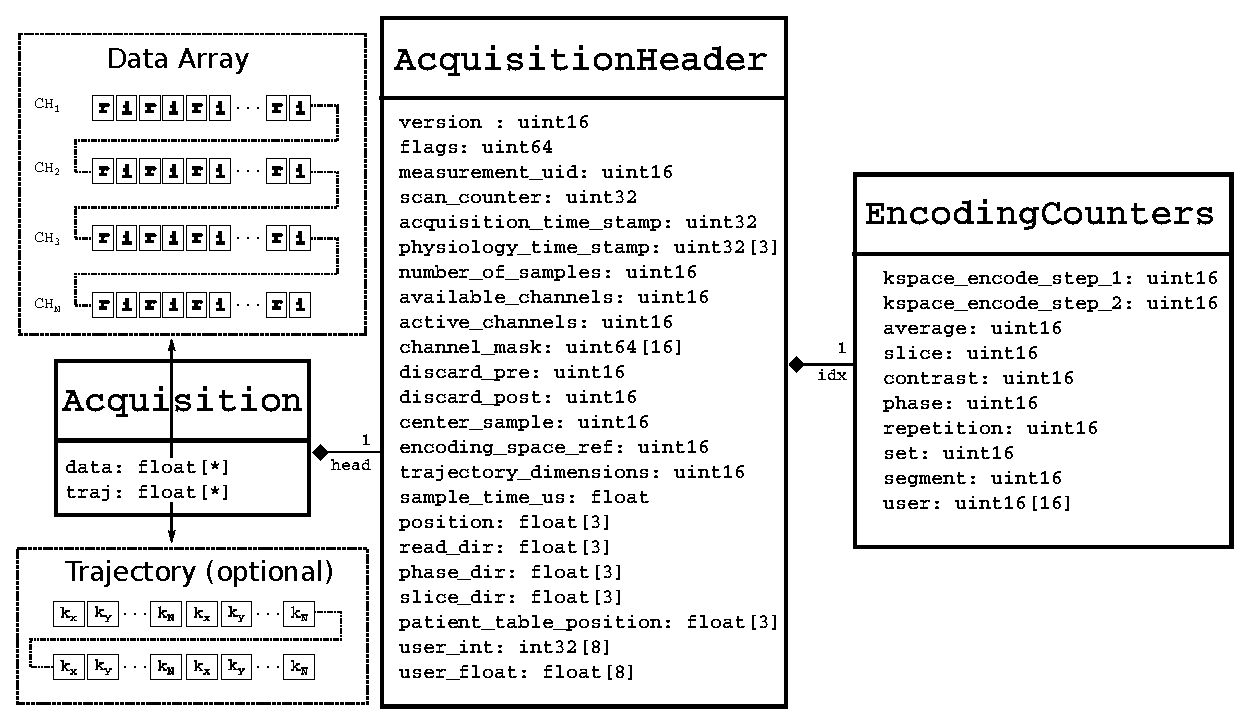
\includegraphics[width=6in]{figure2_uml_diagram.eps}
\caption{Raw data structure for each frame or chunk of the acquisition, consisting of a fixed size header with encoding numbers, location, etc. and the raw k-space data and (optionally) the k-space sampling locations.}
\label{fig:cstruct}
\end{center}
\end{figure}

One of the ISMRMRD file format's key design features is the notion of an ``encoding space" which serves as a description of the type and limits of the experiment and provides the reconstruction program with guidance as to the physical size and resolution of the imaging volume and the ranges of the data header labels.  An ISMRMRD dataset may contain data from several encoding spaces.  Each encoding space is described in the XML header and each acquisition (data chunk) is tagged with a label for the encoding space from which it was acquired. All encoding spaces have a trajectory type, an ``encodedSpace", a ``reconSpace", ``encodingLimits", and an optional trajectory description which can contain an arbitrary set of named parameters like the gradient ramp and flat top times for EPI, or the parameters controlling the shape of the spiral trajectory, etc.  An example of an encoding describing a simple 2D cartesian acquisition is shown in fig.~\ref{fig:encoding}.  In this particular case, the encoding has the following description:
\begin{itemize}
\item the ``encodedSpace" section gives the matrix size ($32\times16\times1$) and field of view in mm ($600\times300\times10$) of the imaging volume encoded by the excitation, i.e. a 10~mm thick slice, 600~mm in x and 300~mm in y, encoded with a nominal matrix size of 32 in x and 16 in y, i.e. at a nominal resolution of 18.75mm.
\item The ``reconSpace" section indicates that the image should be reconstructed on a smaller field of view ($300\times300\times10$), but with half the number of pixels in x.
\item The combination of the ``encodedSpace" and ``reconSpace" indicate that the k-space data were acquired on a grid oversampled by a factor of 2 in the x direction.
\item The ``encodingLimits" section indicates the ky center (5) and the minimum and maximum ky values (0 and 11 respectively), i.e. this is a partial fourier experiment, with a true pixel size that is somewhat larger than the nominal resolution, $min(ky)=-5$, $max(ky)=+6$.
\end{itemize}
% Figure 2
\begin{figure}
\begin{center}
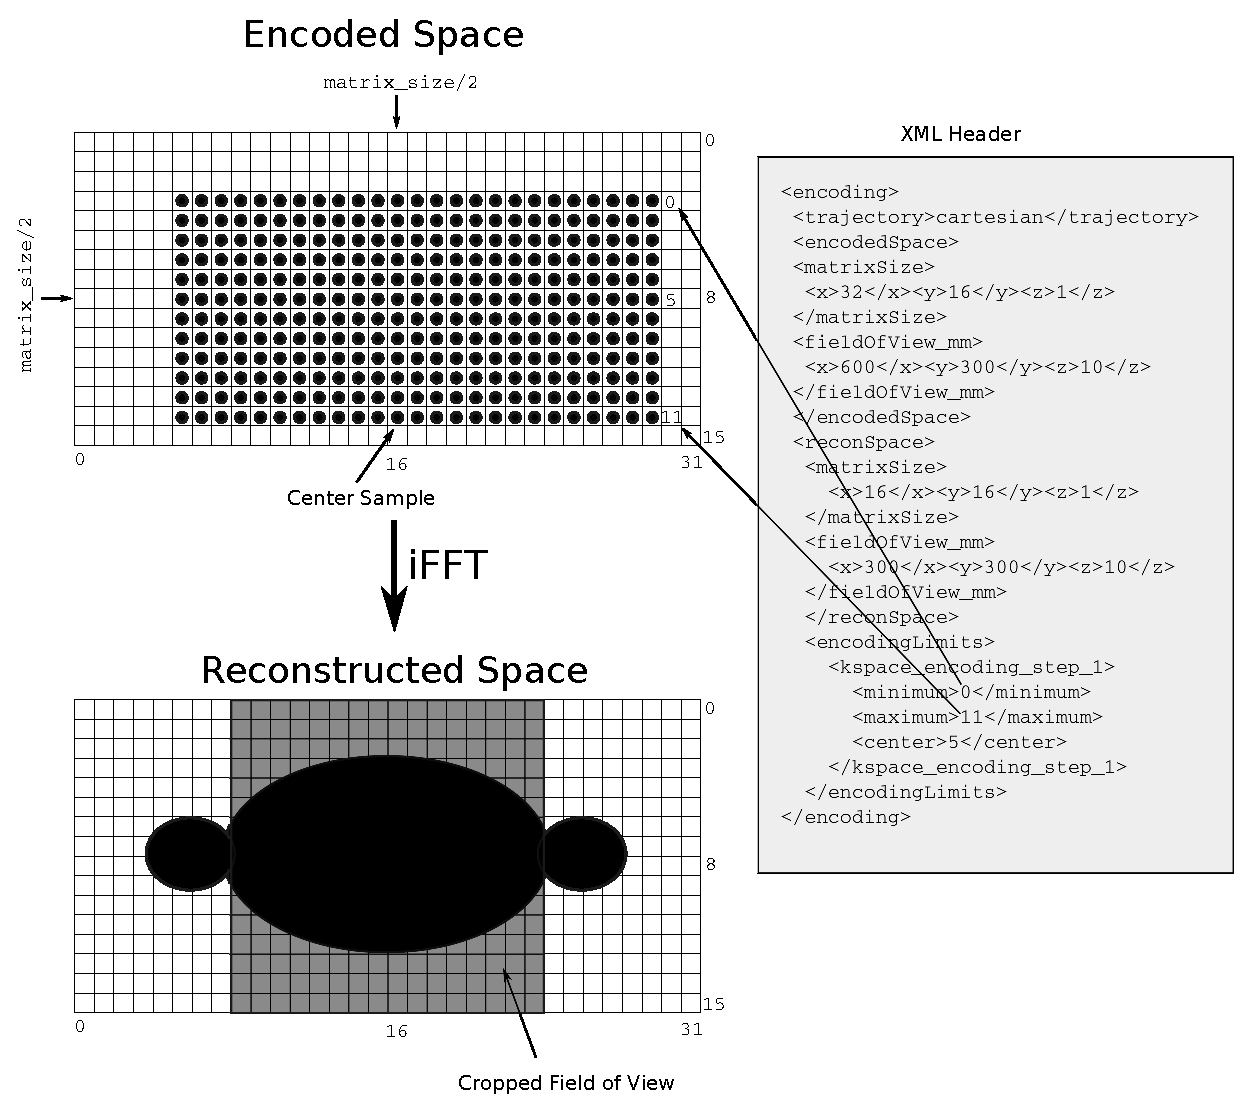
\includegraphics[width=6in]{figure3_encoding_spaces.eps}
\caption{Encoding for a simple 2D cartesian acquisition.  The XML header describes the image encoding and reconstruction fields of view and matrix sizes and k-space sampling bounding box.  The image is acquired at a matrix size of 32 $\times$ 16 $\times$ 1 and field of view of 600mm $\times$ 300mm with a slice thickness of 10mm.  It should be reconstructed at a matrix size of 16 $\times$ 16 $\times$ 1 and field of view of 300mm $\times$ 300mm with a slice thickness of 10mm.   The k-space data were acquired on a grid oversampled by a factor of 2 in the x direction.  The ``encodingLimits" section indicates the ky center (5) and the minimum and maximum ky values (0 and 11 respectively), i.e. this is a partial Fourier experiment, with a true resolution that is somewhat larger than the nominal resolution, $min(ky)=-5$, $max(ky)=+6$.}
\label{fig:encoding}
\end{center}
\end{figure}


\subsection*{ISMRMRD Library}
We have created a cross-platform implementation of this standard using Hierarchical Data Format (HDF) (\url{http://www.hdfgroup.org/HDF5}) files for storage, along with C/C++, Python and MATLAB (Mathworks), libraries for reading and writing ISMRMRD files.  The project follows an open source development model with a website at (\url{http://ismrmrd.github.io}) and a discussion board and code repositories at \url{http://github.com/ismrmrd}.  The library and associated tools can be compiled in a straightforward way on Linux, Windows, and Macintosh computers.  In this section we a provide a high-level description of the implementation and discuss some of the choices we have made during the development process.  The reader is encouraged to examine and experiment with the source code for more a detailed view.

\subsubsection*{Binary file container}
We chose to use HDF as the binary file container.  HDF is very flexible and has been adopted broadly in the scientific community.  Reading and writing from HDF is supported by nearly every programming language and computational environment, in particular it has a core C and C++ API, is supported natively in MATLAB (it forms the basis for MATLAB's own ``.mat" file format), and is supported in Python via the H5Py package (\url{http://www.h5py.org}).

\subsubsection*{Serialization/Deserialization of the XML header}
The XML header can be thought of as a text representation of a flexible binary data structure and although it can be created simply with a text editor (often useful for prototyping), it is usually preferable for the software developer to be able to use the data structure directly and to avoid dealing with the text directly.  Functions to convert between the binary data structure and the text representation reduce error significantly.  The process of generating the text representation from the data structure is usually referred to as ``serialization", and the process of parsing the text representation to populate the fields of the data structure is referred to as ``deserialization".  There are two different strategies for creating the data structure corresponding to the XML structure described by the schema file and to generate the serialization and deserialization functions needed to go between the text and the data structure. One could either: 1) hand craft code, or 2) auto-generate code.  Generally speaking hand crafting code allows for the creation of a better API for the end user, at the expense of (potentially) a great deal of effort on the part of the library authors, whereas auto-generating code is significantly less effort on the part of the library authors, but results in often awkward and inconvenient syntax for the end user. 

\subsubsection*{Three implementations}
In this paper we have used three different programming environments or languages to interact with ISMRMRD files. This section contains a few notes regarding the C/C++, MATLAB, and Python APIs that were created:
\begin{itemize}
\item{XSD Schema.} the file ismrmrd.xsd defines the schema for the XML header.
\item{C library.}  This code defines fixed data structures (ismrmrd.h) and the functions used to interact with the HDF5 file.
\item{C++ library.} This code is a wrapper around the C library with convenience classes and functions that provide memory management and reduce programming error.  It includes a hand crafted XML header binding class.  
\item{Build system.} The C and C++ implementation use the CMake (Kitware) build configuration system in order to support multiple operating systems (Linux, Microsoft Windows, Apple OSX).
\item{MATLAB library.} This code consists of pure MATLAB data structures and functions (classes) which call the MATLAB interface to HDF5 as well as hand crafted Java code for the XML header binding class using the Java provided by MATLAB.
\item{Python library.} This code consists of pure Python classes for the data structures, uses NumPy arrays for the data and the k-space trajectories (\url{http://www.numpy.org}, and an auto-generated XML header binding class.
\end{itemize}

The code repositories also contain the source code for the documentation, Doxygen (\url{http://www.doxygen.org}) and Sphinx (\url{http://sphinx-doc.org}), as well as examples of how to use the APIs to read and write ISMRMRD files.

\subsection*{Vendor Specific Tools}
We have developed converters for several vendors proprietary file formats: Bruker, General Electric, Philips, and Siemens.  The Bruker, Philips and Siemens converters are open source with repositories that can also be found at \url{http://github.com/ismrmrd}.  The GE converter relies on proprietary vendor code and is being distributed via the vendor's research network.  Given the variety in vendor raw data file formats, we  describe the architecture of these programs in general terms in the hope of providing some guidance or aid to others who are implementing their own conversion tools.  We refer the reader to the source code for  details.  Roughly speaking, Bruker raw data is stored in a simple directory structure with the acquisition parameters stored in several text files and k-space data stored in a simple binary file as equal length frames of k-space data (without tags).  Siemens raw data files on the other hand have a more complicated structure.  A single file can store raw data from multiple scans.  For each scan, acquisition parameters are stored in a structured text header, followed by k-space data frames stored in acquisition order, where each frame of k-space data is tagged with a small header containing the frame's line number, slice number, location, etc.  Philips and GE raw data files are organized in structures of intermediate complexity.

The four converters were written in C++.  The acquisition parameters (structured text header or binary data structures) were converted to XML (containing vendor specific parameter names and parameter values).  This XML file was then processed with a sequence specific XSL style sheet to convert the vendor specific parameters into the vendor independent ISMRMRD XML header.  The frames of k-space data were processed in the order in which they appeared on disk.  For vendors with tagged data frames, the proprietary binary header tag was parsed and used to populate the ISMRMRD AcquisitionHeader structure.  For vendors with untagged data frames, sequence and vendor specific knowledge was used.  

It is worth emphasizing that these converters required some work and a good deal of vendor specific knowledge on the part of the developers.  However, once code was developed for converting raw data from one pulse sequence on a particular platform, it was quite straightforward to modify this code to handle other sequences and we believe that others can easily modify these converters to handle currently unsupported product sequences or their own research sequences.

\section*{Experimental Demonstration}
In a typical MR image reconstruction research project, one often tests and validates an algorithm or a particular implementation of an algorithm on simulated data and on data acquired from a phantom or from an in-vivo experiment.  In the interest of reproducible research, a scientist could then distribute the source code and the raw data sets that were used to generate the figures for the publication and perhaps additional code or data related to the testing or validation of the algorithm.

Here we demonstrate how one could use the ISMRMRD format and APIs in such a project: the development, implementation and testing of a trivial image reconstruction algorithm suitable for 2D experiments in which the k-space data are acquired using a multi-channel receiver array and fully sampled on a cartesian grid.  The workflow for this demonstration project is a subset of a more complete full development cycle:
\begin{enumerate}
\item An initial implementation or proof of concept of the algorithm is implemented in a rapid prototyping language such as Matlab or Python.
\item Synthetic data are generated in simulation and used to test/validate the prototype implementation.
\item Real (experimental) data are collected and used to test/validate the prototype implementation.
\item A high performance/production version of the algorithm is implemented in a compiled language such as C/C++ or Fortran.  In some cases the high performance implementation may require specialized hardware such a compute cluster or a graphical processing unit (GPU).
\item The synthetic and real data sets are used to test/validate the high performance implementation of the algorithm.
\item The high performance implementation of the algorithm is put into production in a clinical environment.
\end{enumerate}

% Figure 4
\begin{figure}
\begin{center}
\includegraphics[width=6in]{figure4_recon_demo.eps}
\end{center}
\caption{Experimental demonstration:  Data sets were acquired on scanners from four vendors and converted from the vendor proprietary raw data file formats into ISMRMRD format.  A fifth data set was synthesized numerically and stored in ISMRMD format.  The five ISMRMRD raw data sets were reconstructed using three image reconstruction programs written in C++, Matlab, and Python.  The resulting images are shown above, from left to right Bruker, General Electric, Philips, Siemens, and the synthetic data set,  and from top to bottom C++, Matlab, and Python reconstruction programs.}
\label{fig:demo}
\end{figure}

Our prototypical image research project began with an outline of the steps of the simple 2D image reconstruction algorithm algorithm:
\begin{enumerate}
\item Data are read and stored in a buffer (Nkx,Nky,Ncoil).
\item The fourier transform is computed on two dimensions (x,y).
\item The images are chopped if the data were acquired on an oversampled grid in the frequency encode direction.
\end{enumerate}
The prototype implementation of this algorithm was written in Python (\texttt{do\_recon\_python.py}) and Matlab (\texttt{do\_recon\_matlab.m}).  The high performance implementation of the algorithm was written in C++ (\texttt{ismrmrd\_recon\_cartesian\_2d}).  All three implementations used the corresponding ISMRMRD APIs to read in an ISMRMRD format file and to save the reconstructed image.

A synthetic data set in ISMRMRD format was generated using a program written in C++ (\texttt{ismrmrd\_generate\_cartesian\_shepp\_logan}).  This program simulated a simple experiment collecting data from a single slice object using an 8-element receive array in the presence of a small amount of noise.  The k-space data was generated by multiplying the Shepp-Logan phantom with the receive profile of an 8-rung birdcage coil followed by Fourier transformation and the addition of randomly generated white gaussian noise.

Data sets were collected from a phantom (kiwi fruit) using scanners from four different vendors: 
\begin{itemize}
\item Bruker 4.7T with a single channel 10cm transmit/receive coil
\item GE 3T MR750 with a 32-channel head coil
\item Philips 3T with a 6-channel knee coil
\item Siemens 3T Skyra with a 32-channel head coil
\end{itemize}
Data were acquired using product 2D pulse sequences.  The FOV=10~cm, slice thickness=2~mm, and matrix size (Nx=Ny=512) were matched although no attempt was made to match the pulse sequence type or timings.  The raw data files were transferred off-line and converted into ISMRMRD using the vendor specific converters described above.	

\subsection*{Source Code and Raw Data Dissemination}
The source code for this project is being distributed in several git repositories hosted on GitHub at the URLs listed bellow.  The SHA-1 hashes uniquely identify the particular revision of each of the repositories used for the production of this manuscript:
\begin{itemize}
\item Manuscript LaTeX, figures and Matlab and Python reconstruction: \\
	\url{https://github.com/ismrmrd/ismrmrd-paper} \\
	hash=TBD
\item C++ API and C++ synthetic data generation and C++ reconstruction: \\
	\url{https://github.com/ismrmrd/ismrmrd} \\
    	hash=e7ecb1bbc93c62aceaeb8d197016d67b44e07fee
\item Python API: \\
	\url{https://github.com/ismrmrd/ismrmrd-python} \\
	hash=4e2d8be17ad14fc9ff8d5801751a4511ce435b39
\item Bruker converter: \\
	\url{https://github.com/ismrmrd/bruker_to_ismrmrd}\\
	hash=46dbb5720e9f4304af0920cd6dfa5f7370c75d89
\item GE converter (currently private):\\
	 \url{https://github.com/nih-fmrif/ge-tools} \\
	 hash=f63f74e61e2f8bc920164aa5c8e6ef4dd22705b0
\item Philips converter:\\
	 \url{http://github.com/ismrmrd/siemens_to_ismrmrd}\\
	 hash=5a06e1c5eb3589f650d3c915675a3cab4da0c9e0
\item Siemens converter: \\
	\url{https://github.com/ismrmrd/philips_to_ismrmrd}\\
	hash=b5256ed8267446e70059a5eea88ae6de59c12fe7
\end{itemize}
The raw data in vendor proprietary formats and in ISMRMRD format are being distributed via XNAT (http://central.xnat.org) under the project ``ISMRMRD Paper" with ID ``ISMRMRD".  Readers are encouraged to download the data and source code.

% ------------------------------------------------------------------------
%	Discussion
% ------------------------------------------------------------------------
\section*{Discussion and Conclusion}
We have presented an initial version of a standard for storing raw MR data and have demonstrated an implementation that supports several common programming languages and operating systems. We have also demonstrated that data can be converted to ISMRMRD from common proprietary vendor formats. Once the data has been converted to a vendor independent format, generic reconstruction tools can be used to reconstruct data regardless of the scanner origin. The presented data converters are not complete in the sense that it is be possible to acquire data with any of the vendor platforms that would not yield meaningful ISMRMRD files upon conversion. However, the data converters are either completely available as open source or shared freely in the research communities associated with a specific vendor platform. Following the approach laid out in the source code for the data conversion software it should be a relatively simple task to accommodate other acquisition types. 

In this paper, we focused on 2D cartesian reconstruction examples for simplicity, but more sophisticated reconstruction systems also use the ISMRMRD format. For example, the Gadgetron \cite{Hansen:2013aa} framework uses the format as its internal data representation. The Graphical Programming Interface \cite{Zwart:2014aa} has also been used with the ISMRMRD format using a set of externally provided compute nodes (\url{https://github.com/hansenms/gpi_ismrmrd})

Future work will be focused on expanding the header sections in the flexible XML header to support specific applications.  Future changes to the fixed memory layout (C-struct) header and data may include capabilities to store arbitrary waveform data elements that could be used to capture detailed information about gradient waveforms or physiological telemetry. 

We believe that as this standard is refined and evolves it will serve as a foundation upon which practitioners can base reproducible research project and collaborations.  A great deal of work remains and we ask for input from the ISMRM community to help shape the direction of the format. Specifically, the project would benefit from volunteers that have a very detailed understanding of more specialized research applications and their requirements in terms of which experimental details need to be captured to produce high quality reconstructions. We would also like to encourage groups with existing software packages to adopt this open data format as one of the input formats they support. 

It is important to reiterate that the ISMRMRD format is a completely open and community driven format. The authors and developers would like to invite anybody in the community (including commercial vendors) to participate either as users of the format or as developers of the format or associated tools.

% ------------------------------------------------------------------------
%	Acknowledgments
% ------------------------------------------------------------------------
\section*{Acknowledgements}
Multiple people participated in the discussions that led to this work.  We would like to acknowledge their contribution (in no particular order) 
Walter F. Block,
Peter Boernert,
David O. Brunner,
Mark A. Griswold,
Brian A. Hargreaves,
Craig H. Meyer,
Sonia Nielles-Vallespin,
Tim Nielsen and 
Douglas C. Noll.


% ------------------------------------------------------------------------
%	References	
% ------------------------------------------------------------------------
\bibliography{ismrmrd}

\end{document}
